\section{Notas, promedios y archivos}

Se tiene un archivo \texttt{notas.txt} con la estructura \texttt{nombre\#ramo\#notas} donde notas está separado por el string \texttt{";"}.

\begin{center}

\begin{tabular}{|l|}
    \hline
    \texttt{notas.txt} \\ 
    \hline
    anghelo\#mat021\#76;78;54 \\
    miguel\#mat021\#80;56;67 \\
    miguel\#fis100\#95;86;75 \\
    diego\#iwi131\#100;99;98 \\
    \hline
\end{tabular}
\end{center}

% \begin{figure}[h]
%     \centering
%     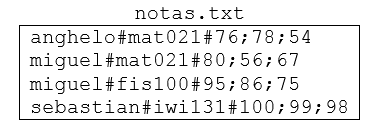
\includegraphics{Imagenes/notas1.PNG}
% \end{figure}

Se le pide a usted programar las funciones:

\begin{itemize}
    \item[a)] \texttt{alumnos\_ramo(archivo,ramo)} que retorne un entero con la cantidad de alumnos que rindieron \texttt{ramo}.
    
    \begin{lstlisting}[style=consola]
>>> alumnos_ramo('notas.txt','mat021')
2
    \end{lstlisting}
    
    \item[b)] \texttt{promedio\_ramo(archivo,ramo)} que retorne un entero con el promedio de \texttt{ramo}.
    
        \begin{lstlisting}[style=consola]
>>> promedio_ramo('notas.txt','mat021')
68
    \end{lstlisting}
    
    \item[c)] \texttt{agregar\_promedio(archivo)} que agregue al final de cada linea el promedio del ramo de cada sujeto, separado con un gato \texttt{"\#"}. La nota ingresada final debe ser un numero entero.
    
    
\begin{center}


\begin{tabular}{|l|}
    \hline
    \texttt{notas.txt} (luego de la función \texttt{agregar\_promedio()}) \\
    \hline
    anghelo\#mat021\#76;78;54\#69 \\
    miguel\#mat021\#80;56;67\#67 \\
    miguel\#fis100\#95;86;75\#85 \\
    diego\#iwi131\#100;99;98\#99 \\
    \hline
\end{tabular}
\end{center}

% \begin{figure}[h]
%     \centering
%     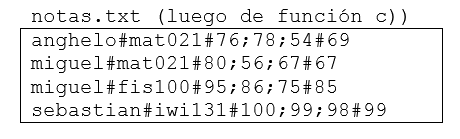
\includegraphics{Imagenes/notas2.PNG}
% \end{figure}

\end{itemize}
